In this section we will provide and overview of the relevant background and context for this thesis. First introducing the software engineering lifecycle and the rising role of GenAi/LLMs in it. The Second part showcases the evolution and state of APR and explores existing approaches.

\section{Software Engineering}
In the follwing section introduces the software engineering lifecycle, the role of code hosting platforms, and the importance of Continuous Integration and Continuous Deployment (CI/CD) in modern software development.
\subsection{Software Development Lifecycle}
Engineering Software is complex and including multiple stages. For structuring this work diffrent Software Developemnt Lifecycle Models have been introduced. Software Development Lifecycle Models evolve constantly to adapt to the chanign needs of creating software. The most promising and widely used model is the Agile Software Development Lifecycle \cite{rupareliaSoftwareDevelopmentLifecycle2010}.

The Agile lifecycle brings an interative approach to development, focusing on collaboration, feedback and adaptivity. The Goal frequent delivery of small functional features of software, allowing for continuous improvement and adaptation to changing requirements. Agile can be used with multiple frameworks like Scrum or Kanban but follows a similar approach. \cite{rupareliaSoftwareDevelopmentLifecycle2010}.

\begin{figure}[htbp]
    \centering
    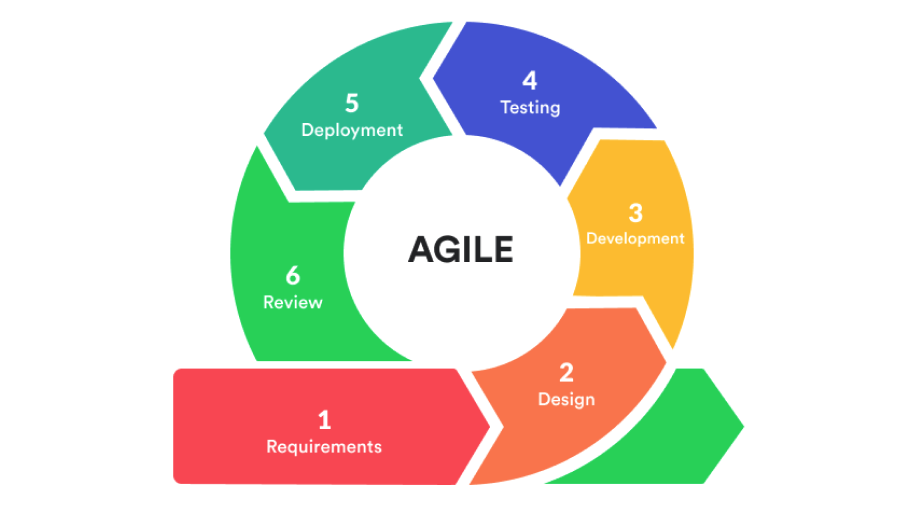
\includegraphics[width=0.8\textwidth]{images/agile-cycle.png}
    \caption{Agile Software Development Lifecycle}
    \label{fig:agile-cycle}
\end{figure}

A Agile Software Development Lifecycle iteration consists of several key stages like in Figure starting with planning phase where requirements for the iterartion are gathered and pritorized.

Since agile focuses adaptivity arising bugs can alter iterations if priotirised and therefore slow down delivery of features. APR is supposed to help with this problem by accelerating the process of fixing bugs.
---explain how bugs are handled

Software development is moving towards lightly coupled microsversives which results in more repositories which are smaller in scale tailored towards a specialzed domain. This trend is driven by the need for flexibility, scalability, and faster development cycles. Smaller code repositories allow teams to work on specific components or services independently, reducing dependencies and enabling quicker iterations. This approach aligns with modern software development practices, such as microservices architecture and agile methodologies.
With this trend developers work on multiple projects at the same time, which can lead to more interrupptions and context swtiching when problems arise and priorities shift.


\subsection{Continuous Integration}

For accelerating the delviery of software in an iteration continous integration has become a standard in agile software development.

\begin{figure}[htbp]
    \centering
    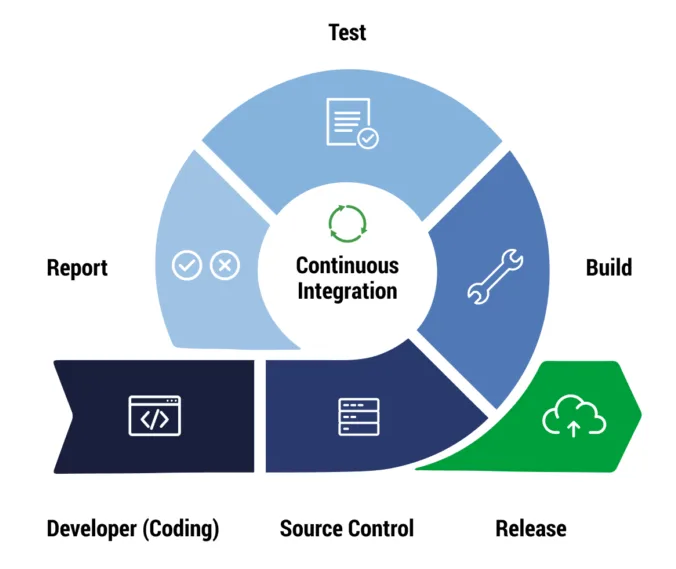
\includegraphics[width=0.8\textwidth]{images/ci-cycle.png}
    \caption{Continuous Integration Cycle}
    \label{fig:ci-cycle}
\end{figure}

Continuous Integration (CI) allows for frequenct code integration into a code repository. Ci can integrate steps like automated building and testing into the development resulting in rapid feedback right where the changes commited to the shared reposirotry.

Althought CI bring a lot of potential to development it can also have problemswhich can be long build durations and high maintance

CI supports aspects like fast delivery, fast feedback, enhanced collaboration which are ciritcal for agile software development. \cite{ugwuezeContinuousIntegrationDeployment2024}

\subsection{Software Project Hosting Platforms}
Software projects are hosted on platforms like Github or gitlab. With Github being the most popular and most used \cite{} These platforms provides tools and feature for the complete software development lifecycle. Project hosting, verssion control, bug and issue tracking, project management, backups, collaboration, and documentation. \cite{abrahamssonAgileSoftwareDevelopment2017}

GitHub has features like Issue tracking for requiremtns and planning with issues looking like this: \cite{githubdoc}
---image of issue
has title, description, comments, labels and mroe assioicated information

also provides a manged soltution for integrating CI into reposiries by writing workflows in YAML files called Github Actions. The pipeliens can run on github hosted runners or self hosted runner. A workflow can be triggered by one or more event. One or more jobscan be executed on a provided runner maschiene. A job can consist of multiple steps. \cite{Workflows}
\begin{figure}[htbp]
    \centering
    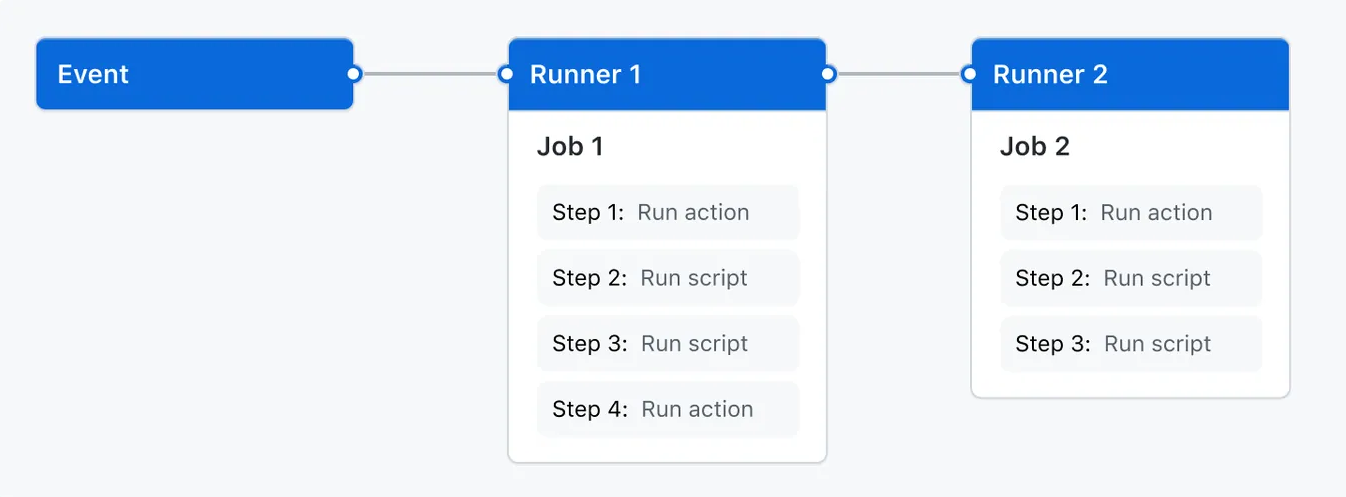
\includegraphics[width=0.8\textwidth]{images/overview-actions-simple.png}
    \caption{Simple Action}
    \label{fig:simple action}
\end{figure}

Since constant feedback and reviews of code play an imporatnt role in agile workflows github also provides a pull request feature. Pull Requests allow for proposal of changes to the codebase, with an integrated review process which allows for collaboration and review before changes are integrated into the production codebase. This process is essential for maintaining code quality and ensuring that changes are thoroughly vetted before being merged into the main branch. \cite{githubdoc}

\section{LLMs in Software Development}
Generative AI is reshaping software development by autoamting various tasks. Modern large language models have billions of paramters, are pre-tained on massive codesbases which results in extraordinary capbilites in this area  \cite{chenUnveilingPitfallsUnderstanding2025}.
Therefore LLMs get applied in generating code, debugging, refacting and testing. \cite{sauvolaFutureSoftwareDevelopment2024,bhargavmallampatiRoleGenerativeAI2025} By using LLMs to enhance these tasks developemtn cycle times can be reduced by up to 30 percent \cite{bhargavmallampatiRoleGenerativeAI2025}.
Tools like Github Copilot, OpenAI Codex, and ChatGPT have become popular in the software development community, providing developers with AI-powered code suggestions and completions for dirrent tasks \cite{bhargavmallampatiRoleGenerativeAI2025}.

Still Problems exsist as Gneerative Ai:
is very researouce intensive
eithical diellemas and interlecutal property issues \cite{sauvolaFutureSoftwareDevelopment2024}


Problems with llms when genrating code are: Information leakage, hallucinations, and security issues

now research is looking into developing and improving specialized workflows leveraging LLMs \cite{puvvadiCodingAgentsComprehensive2025}.

recently mroe attention is given to itnergration of AI/ML into CICD
\cite{mohammedAIDrivenContinuousIntegration2024} and integrating into exising workflows \cite{sauvolaFutureSoftwareDevelopment2024}

\section{Automated Programm Repair}

Automated Program Repair (APR) is software that helps detect and repair bugs in code with minimal human intervention. This field has also benefited of the rapid advancements in AI.

APR system are supposed to take over the process of fixing bugs therefore making more time for developers to focus on more relevant work. 
localization, repair, and validation


\subsection{Evolution of Automated Program Repair}
APR was first introduced in xxx and has come a long way since then.
% TODO cite 
Earliest APR techniques were based on version control history, using the history to roll back to a previous version of the code part, where no issues were present. This approach, while effective in some cases, often lacked the ability to perserve new features. (more like instant rollback)
history based

--- search based repair,

---semantic based repair,

---tempalte based repair,
apply predefined transformtions to the code based on rules

---The emerge of llm based techniques
LLM based APR techniques have demonstrated siognificant uimrpovemetns over all other state of the art technqiues, benfitintting from theor coding knowledge \cite{hossainDeepDiveLarge2024}

Agent Based
agent based system improve fixing abilites by probiding llms the ability to interact with the code base and the environment, allowing them to plan their actions  \cite{yangSWEagentAgentComputerInterfaces2024}.

llms lay the groundwork of a new APR paradigm \cite{chenUnveilingPitfallsUnderstanding2025}

complex agent arcitectures produce good results espically paired with containerized environments. Emphasis on quality insureance and Devops practices \cite{puvvadiCodingAgentsComprehensive2025}


modern aprs usally consist of multiple stages, including localization, repair, and validation. These stages are often implemented as separate modules, allowing for flexibility and modularity in the repair process \cite{yangSWEagentAgentComputerInterfaces2024}.

recently a push towards more lightweight approaches has emerged, focusing on simplicity and efficiency. These approaches aim to reduce the complexity of APR systems while maintaining effectiveness in bug fixing \cite{xiaAgentlessDemystifyingLLMbased2024}.

\subsection{Related Work - Existing Systems}


end to end without llms Sapfix from Facebook. Fixing bugs in production envrioments lowerring incidents mean time of recovery significantly \cite{margineanSapFixAutomatedEndtoEnd2019}

FixAgent \cite{leeUnifiedDebuggingApproach2024}

swe agent \cite{yangSWEagentAgentComputerInterfaces2024}

Agentless minimal system \cite{xiaAgentlessDemystifyingLLMbased2024}
claims exsiting systems are too complex and compute/costs intensive.
lacks the ability to control the decision planning.
they use a minimalist approach using localization, repair and validation.


this appraoch inspried the thesis to test how a simple approach will perform in a real world scendario on a code hosting platform.


--point out areas where current systems see limitation

-- during the research for this thesis, full integrations where published by companies like OpenAI Codex and Github Copilot - but these are not open source


\subsection{APR in CI Context}

CI allows seemless integration...
this way there is no harmfull code executed on own machiene, its encapsulated mutliple times container in Ci runner
